\documentclass[a4paper]{article}
\usepackage[utf8]{inputenc}
\usepackage{geometry}
\usepackage{graphicx}

\usepackage[T1]{fontenc}
\usepackage{lmodern}
\usepackage[ngerman]{babel}

\usepackage{float}

\usepackage[colorlinks,
pdfpagelabels,
pdfstartview = FitH,
bookmarksopen = true,
bookmarksnumbered = true,
linkcolor = black,
plainpages = false,
hypertexnames = false,
citecolor = black] {hyperref}

\usepackage[nottoc]{tocbibind}

\title{Projektdokumenation\\Web-basierte Anwendungen\\Verteilte Systeme}
\author{Dennis Meyer\\Dominik Schilling}
\date{\today}

\begin{document}

\maketitle

\newpage

\tableofcontents

\newpage


\section{Einleitung}
Im Rahmen der Projektphase des Moduls Webbasierte Anwendungen 2: Verteilte Systeme, geht es um die Entwicklung einer Applikation, die sich mit dem Datenaustausch in verteilten System beschäftigt. Innerhalb dieses Systems wird zum einen eine synchrone Kommunikation zwischen Instanzen mit Hilfe des REST Konzeptes realisiiert und zum andern ein asynchroner Datenaustausch auf Grundlage von XMPP. TODO


\section{Konzept}

Die \textbf{Idee} ist, dass Serien-Interessierte über ihre zuvor favorisierten Serien und abonnierten Interessen benachrichtigt werden, sobald eine Episode dieser Serie im TV ausgestrahlt wird.

\parskip 12pt
\parindent 0pt
Der \textbf{Serien-Interessierte} soll Zugriff auf einen Pool von Serien bekommen, die auf einem Server gespeichert und verwaltet werden.
Die einzelnen Serien soll der Nutzer dann favorisieren/abonnieren können um dann über die TV-Ausstrahlung informiert zu werden.
Außerdem soll die Möglichkeit bestehen eine Episode zu bewerten und als gesehen/ungesehen zu markieren. Es besteht zudem die Möglichkeiten Serien in Listen einzuordnen und zu verwalten. (definitiv automatische Watchlist/Seenlist)

\parskip 12pt
\parindent 0pt
Die \textbf{Server-Anwendung} soll die Nutzer über die TV-Austrahlung einer Episode einer zuvor favorisierten Serie in einem vom Benutzer definierten Zeitraum informiert werden. Jeder Eintrag einer Serie enthalt zudem Informationen wie Genre, anhand derer Abonnentenl bezüglich eines bestimmten Themas, zusätzliche Benachrichtigungen empfangen.

\parskip 12pt
\parindent 0pt
Ein \textbf{Content-Admin} soll erweiterte Rechte bekommen, um die Content-Verwaltung zu übernehmen. Die Anwendung soll das Anlegen, Bearbeiten und Löschen von Serien bzw Episoden ermöglichen. Zudem ist somit das Korrigieren von Fehlern möglich, die von Usern eingeschickt werden.

\subsection{Zusatz - Freunde}
Serien-Interessierte sollen sich gegenseitig hinzufügen/abonnieren können um sich gegenseitig zu benachrichtigen, zum Beispiel in Form von Freund X schaut gerade Y, Freund Z hat Serie/Episode mit 8,0 bewertet oder Freund Y empfiehlt Dir Serie W.


\subsection{Umsetzung}
Die Anwendung ermöglicht den Austausch von Informationen zwischen Server und Anwender entsprechend den jeweiligen Funktionen.

\subsubsection{Synchrone Datenübertragung}

Zum einen hat der Anwender direkt die Möglichkeit auf Informationen in Form von Daten zuzugreifen und diese zu Manipulieren.

\begin{itemize}
\item
Serien-Interessierte
	\begin{itemize}
	\item
    Markieren von Episoden
    	\begin{itemize}
    	\item
     	Gesehen/Nicht gesehen
     	\end{itemize}
    \item
    Bewertung einer Episode
      	\begin{itemize}
      	\item
        Kommentar
        \item
        Bewertung in Zahlen
        \end{itemize}
     \item
     Fehlermeldung
     	\begin{itemize}
     	\item
        geänderte Sendezeit, fehlerhaftes Datum
        \end{itemize}
     \item
     Listen
     	\begin{itemize}
     	\item
    	Ausgabe (Un)Watched
    	\item
     	Ausgabe vorhandene Serien
     	\item
     	Ausgabe Follower/Following (?)
     	\end{itemize}
     \item
     Favorisierung
   	  	\begin{itemize}
   	  	\item
   	  	Anlegen
   	  	\item
   	  	Löschen
   	  	\item
   	  	Bearbeiten
   	  		\begin{itemize}
   	  		\item
   	  	    Zeitpunkt der Benachrichtigung
   	  	    \end{itemize}
		\end{itemize}
	\end{itemize}
	\item
	Content-Admin
		\begin{itemize}
		\item
		Verwaltung der Episoden
			\begin{itemize}
			\item
			Anlegen
			\item
			Löschen
			\item
			Bearbeiten
			\end{itemize}
		\end{itemize}
\end{itemize}


\subsubsection{Asynchrone Datenübertragung}

Ein weiterer Aspekt ist das Anfordern von Informationen, wobei die entsprechenden Informationen von Seiten des Servers von Bedingungen abhängig gesendet werden, was auch mehrfach geschehen kann.

\begin{itemize}
\item
Serien-Interessierte
	\begin{itemize}
	\item
    Benachrichtung bei TV-Austrahlung
    \item
    Freunde mit gleicher Favorisierung bei Serienstart mit Check-in benachrichtigen (?)
	    \begin{itemize}
	    \item
         Freund X schaut auch W
         \end{itemize}
    Empfehlung einer Serie von Freund(e) anzeigen (?)
    \end{itemize}
\item
Content-Admin
	\begin{itemize}
	\item
    Benachrichtung bei Fehlermeldung durch User
    \end{itemize}
\end{itemize}



\begin{figure}[H]
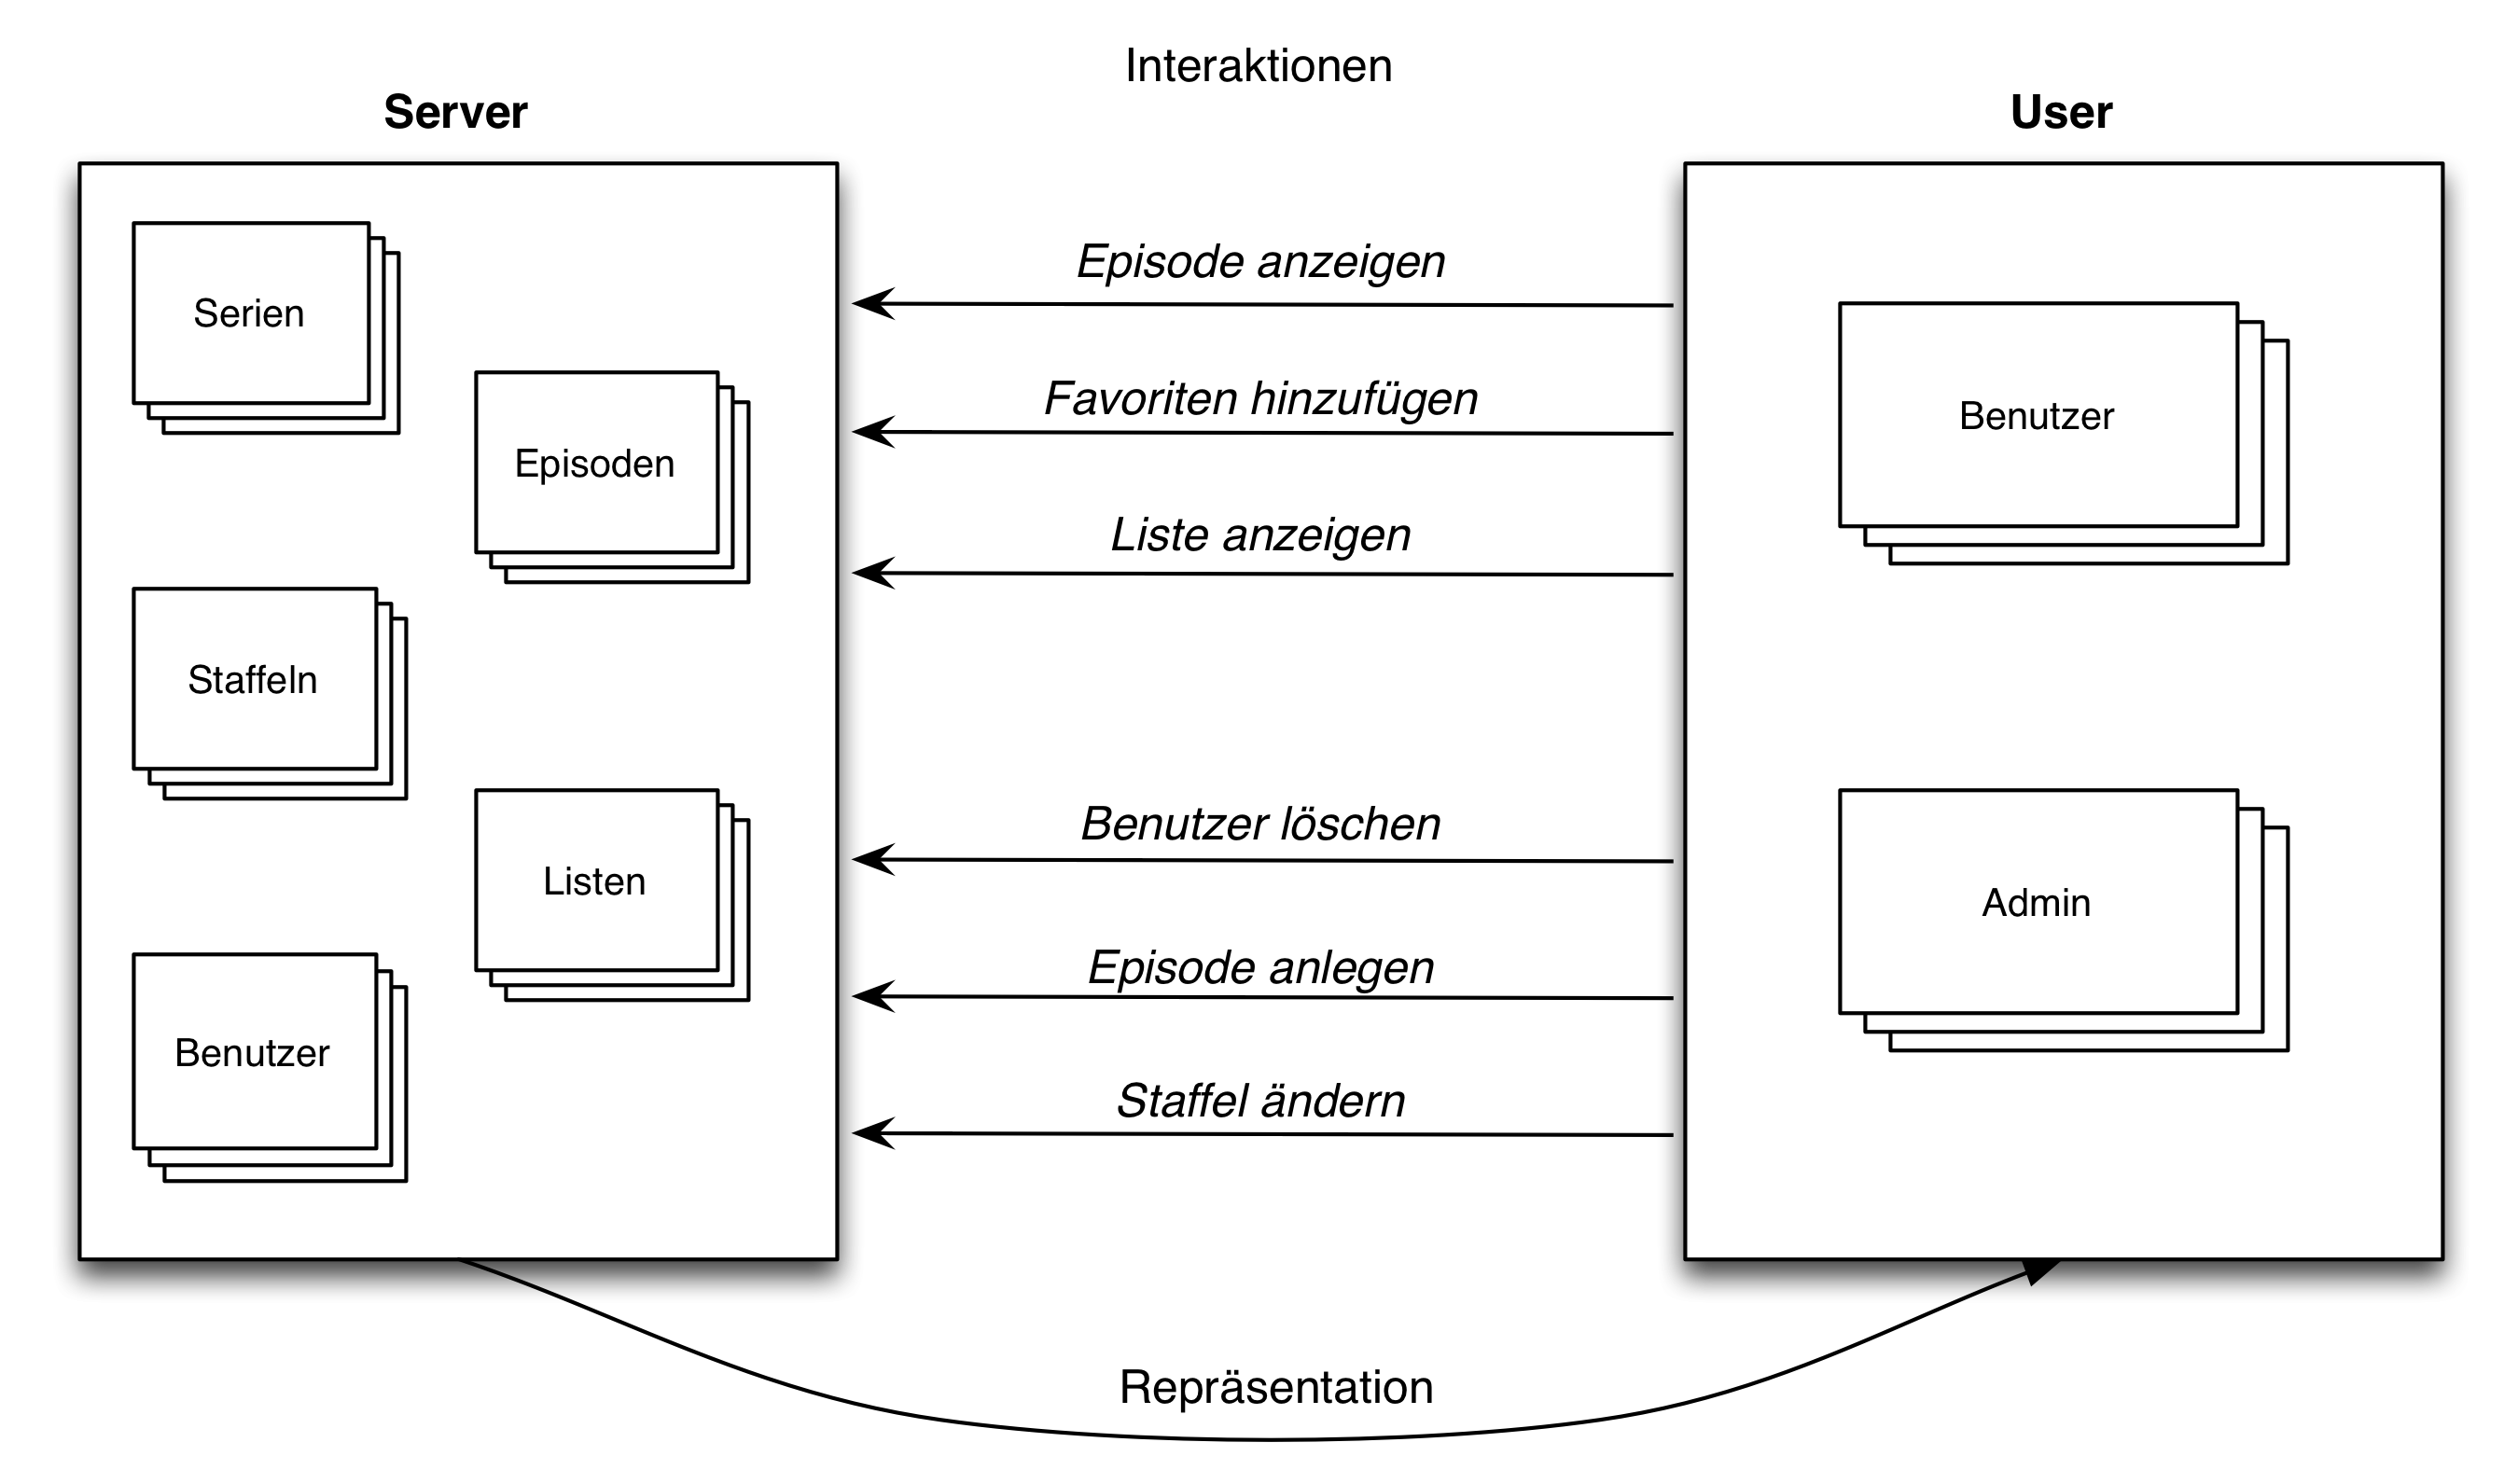
\includegraphics[width=1\textwidth]{images/kommunikationsablaeufe.png}
\caption{Synchrone Kommunikationsabläufe}
\label{kommunikationsablaeufe}
\end{figure}


\begin{figure}[H]
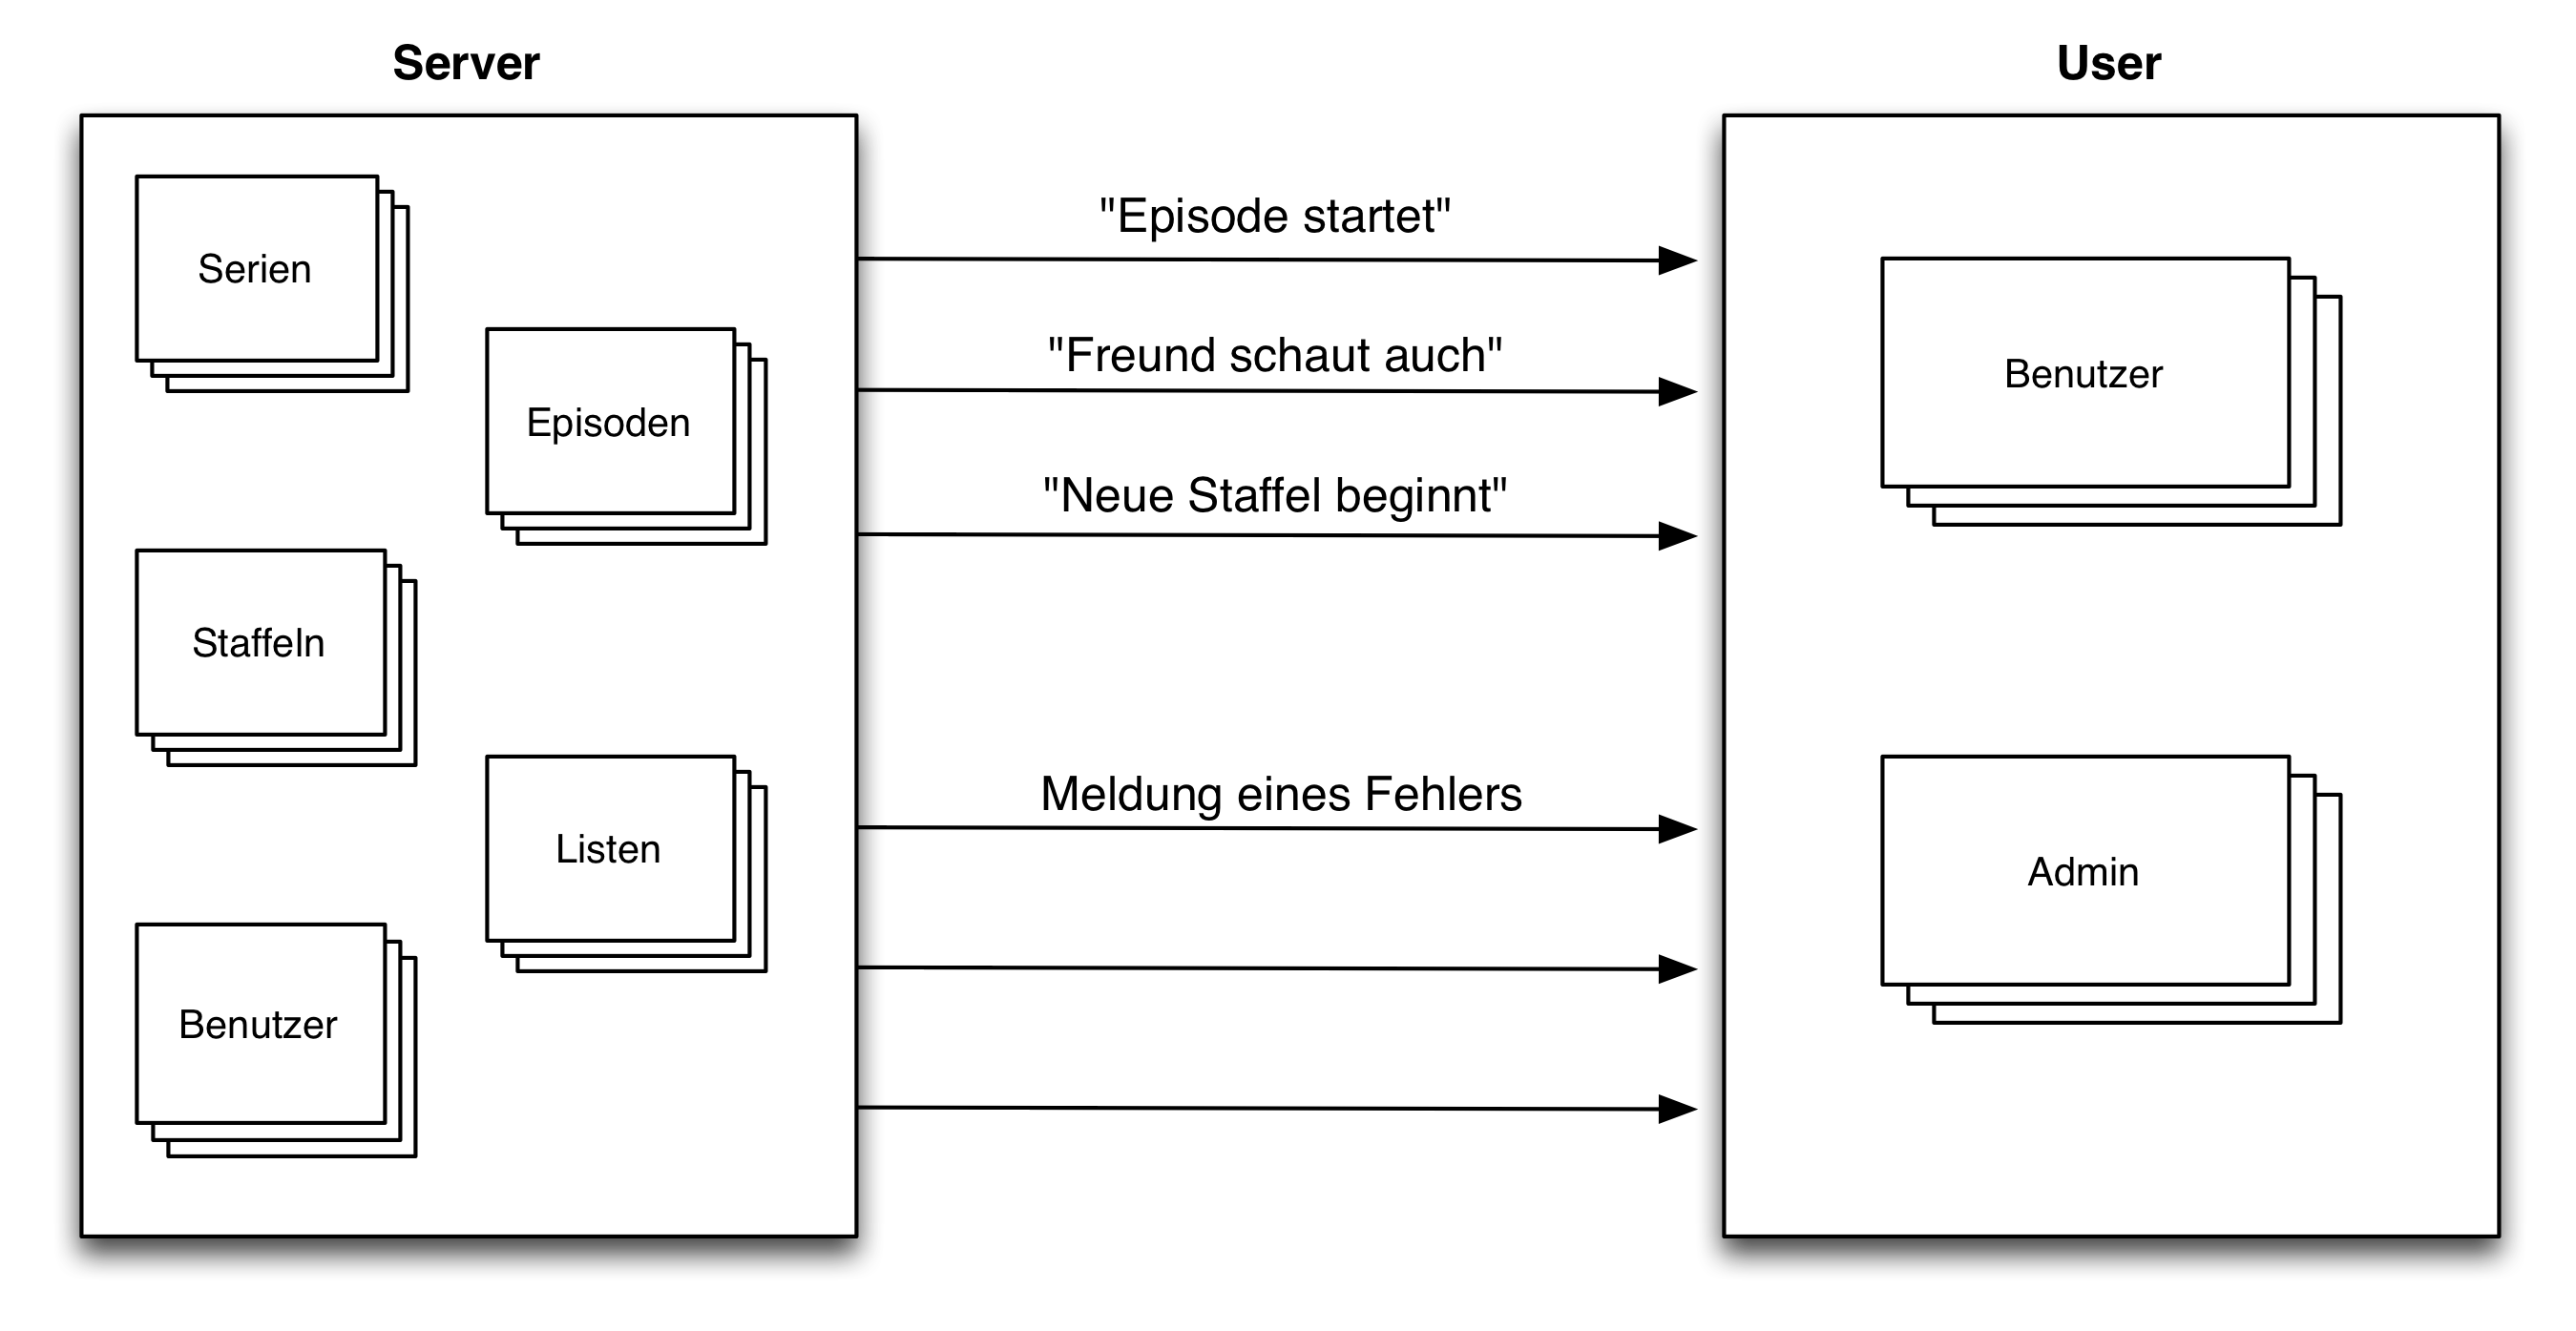
\includegraphics[width=1\textwidth]{images/kommunikationsablaeufeAsynchron.png}
\caption{Asynchrone Kommunikationsabläufe}
\label{kommunikationsablaeufeAsynchron}
\end{figure}


\newpage

\section{Entwicklung des Projektes}

\subsection{Projektbezogenes XML Schema / Schemata}
\subsubsection{Vorüberlegungen}
Der erste Meilenstein befasst sich mit der Repräsentation von Daten in XML.

Damit bei der Verwendung der XML Dateien bei der späteren Verarbeitung mit JAXB keine Probleme auftreten,
ist es notwendig eine Validierung der Dateien durch Definition zugehöriger XML Schemas durchzuführen.
Vorteil bei der Verwendung eines Schemas ist, neben der Kontrolle auf Wohlgeformtheit und der Verwendung
definierter Datentypen und Strukturen, auch das festlegen von Restriktionen.

Hinsichtlich des zugrunde liegenden Konzeptes und den benötigten Informationen, gibt es viele Elemente
innerhalb der Dateien, die nur mit Strings realisiert werden können. Das Problem bei freier Definition
besteht darin, dass die Datensätze sehr fehleranfällig sind, wenn es um die Benutzung durch Menschen geht.
Rechtschreibfehler beim Namen des Landes, des Fernsehsenders oder des Genres, würden für den Leser bzw.
Interessenten der Anwendung noch kein Problem darstellen, da er vermutlich deuten könnte was gemeint ist.
Informationstechnisch ist es aber von Vorteil, die Datensätze möglichst konsistent und reichhaltig anzulegen.

Das System des Serientrackers beruht darauf, die Verwaltung von Serien anhand von Listen und Tags wie
Gesehen, Ungesehen zu ermöglichen. Wie bereits in der Besprechung der Umsetzung erwähnt, wird anhand
dieser Informationen auch die Asynchrone Datenübertragung realisiert.
Das Abonnieren von Informationen zu laufenden Serien des Genre Krimi, greift bei Benachrichtigung auf
Datensätze zu, die diesem Elementwert unter dieser eindeutigen Zeichenfolge zugeordnet sind. Formulierungsfehler
wie Krimie oder Crime, führen dementsprechend zu Komplikationen, weil sie die Konsistent der Informationssätze beschädigen.

Die Auseinandersetzung führte zu dem Ergebnis, dass folgende Objekttypen innerhalb des Serientrackers von interesse sind und wiederkehrende Elemente darstellen:

Serie \\
Eines der wichtigsten Elemente, dass alle Informationen beinhaltet, die für den Benutzer von bedeutung sind, ist die Serie. 
Eine Serie besitzt allgemeine Informationen wie Name, eine Beschreibung, der Sender indem sie ausgestrahlt wird oder das Produktionsland.
Im realen Kontext wird eine Serie zudem in Staffeln ausgestrahlt, die jeweils eine bestimmte Anzahl von Episoden enthalten.

Staffel \\
Bestandteil einer Serie, von der es im Laufe der Jahre immer neue Objekte gibt und die nach einer gewissen Anzahl an Episoden als abgeschlossen gelten.

Episode \\
Ein Kernelement des Systems, dass ein wichtigen Typ für die asynchrone Kommunikation darstellt. Durch das Abonnieren von Genres oder Serien, wird die Benachrichtigung in Bezug auf eine einzelne Episode ausgelöst, die sich durch ihr jeweiliges Austrahlungsdatum und -zeitpunkt kennzeichnet. 
Zudem kann der Inhalt der Episode von Interesse sein.

User \\
Neben den Serieninformation, gibt es die Anwender des Serientrackers, die sich anmelden und durch Listen die Dienste des Serientrackers abonnieren.
Allgemein werden hierbei personenbezogene Daten wie Username und echter Name erwartet, so wie Zusatzinformationen, die für andere Benutzer von Interesse sein könnten und die Person hinter dem Profil genauer beschreiben. Beispiele wären das Alter, ein Profilbild, Wohnort oder eine kurze Beschreibung.

Liste \\


Als zusätzlicher Typ, der jedoch erst in der asynchronen Kommunikation verwendung finden wird, wurde die Message, also eine bestimmte Art von Nachricht identifiziert.

Für diese Obertypen gilt es ein valides XML Schema zu definieren, wobei während der Entwicklung verschiedene Aspekte betrachtet werden müssen.  

\newpage

\subsubsection{Datentypen}
Bei der Definition eines XML Schemas, sollte neben der enstprechenden Datensatzstruktur auch festgelegt werden, durch welche Datentyp die einzelnen Informationen repräsentiert werden sollen.

\newpage

\subsubsection{Restriktionen}
Um die eingegeben Daten semantisch sinnvoll zu halten, wurde für einige Elemente und Attribute Bedindungen hinzugefügt, die im jeweiligen Zusammenhang sinnvoll erscheinen. 

\begin{table}[H]
\caption{Restriktionen des User Schemas}


\begin{tabular}{l l l}
\\ [-0.5ex]

\hline\hline
\\ [-0.5ex]
Element/Attirbute & Restriktion & Begründung
\\ [1.5ex]
\hline
\\ [-0.5ex]
Username & Stringlänge 2 < und < 30 & sinnvolle Namenlänge, verhindert Text \\[1ex]
Lastname & Stringlänge 1 < und < 40 & gängige Nachnamenlänge, eventuell Doppelnamen,\\[1ex]
&&verhindert Text \\[1ex]
Firstname & Stringlänge 1 < und < 50 & gängige Vornamenlänge, Mehrfachnahmen \\[1ex]
Gender & Auswahl zwischen Male und Female & logische Auswahl, Vorgabe verhindert \\[1ex]
&&Schreibfehler durch User\\[1ex]
Age & älter als 13 und jünger als 121 & Mindestalter zur rechtlichen Nutzung, \\[1ex]
&&Alter nach oben sinnvoll begrenzt \\[1ex]
Location & Stringlänge < 40 & Stadtname, Land etc. Eingabe ist keine Adresse\\[1ex]
&&und lässt sich in Kürze ausdrücken\\[1ex]
About & Stringlänge < 200 & optionale Kurzbeschreibung, nach oben begrenzt, \\[1ex]
&&zu viele Informationen nicht unbedingt von Interesse  \\[1ex]
Admin & Boolean ob True or False & Rechtevergabe nach Status,\\[1ex] 
&&Auswahl nur in 2 Zuständen möglich\\[1ex]

\hline
\end{tabular}
\label{tab:restriktionenderxsd}
\end{table}


\begin{table}[H]
\caption{Restriktionen des Serie Schemas}


\begin{tabular}{l l l}
\\ [-0.5ex]

\hline\hline
\\ [-0.5ex]
Element/Attirbute & Restriktion & Begründung
\\ [1.5ex]
\hline
\\ [-0.5ex]
Year & Jahreszahl 1900 < und < 2015 & Jahreszeiten außerhalb unrelevant \\[1ex]
Country & Auswahlmöglichkeit Ländern, die Serien produzieren & verhindern von Eingabefehler der User\\[1ex]
Episoderuntime & Auswahl zwischen gängigen Episodenlängen& Serie hat feste Episodenlänge, bekannte Längen \\[1ex]
Network & Auswahl bekannter Sender & unrelevante Sender entfallen, Eingabefehler verhindern \\[1ex]
Airday & Auswahl des Tagnamen & Eingabefehler verhindern \\[1ex]
Genre & Auswahl definierter Genres & einheitliche Schreibweise, Eingabefehler verhindern, sinnvolle Genre\\[1ex]

\hline
\end{tabular}
\label{tab:restriktionenderxsd}
\end{table}




\begin{table}[H]
\caption{Weitere Restriktionen}


\begin{tabular}{l l l}
\\ [-0.5ex]

\hline\hline
\\ [-0.5ex]
Element/Attirbute & Restriktion & Begründung
\\ [1.5ex]
\hline
\\ [-0.5ex]
Overview (global) & Stringlänge 10 < und < 500 & Vermittlung von allgemeinen Informationen,\\[1ex]
 &&kurze Inhaltsangabe \\[1ex]
Title (global) & Stringlänge 1 < und < 80 & gängige Titellänge \\[1ex]
Name (list) & Stringlänge 2 < und < 80 & treffende Bezeichnung, Name keine Beschreibung \\[1ex] 
Public (list) & Boolean True und False & feste Zustände \\[1ex] 
Episodenumber (episode) & Anzahl < 26 & maximale Episodenanzahl pro Season gängiger Serien \\[1ex] 
Seasonnumber (seasons) & Anzahl < 41 & sinnvolle Begrenzung, Freiraum für Langzeitserien \\[1ex] 

\hline
\end{tabular}
\label{tab:restriktionenderxsd}
\end{table}

Neben diesen Restriktionen einzelner Elemente bezogen auf ihre Werte, bestehen auch Genehmigungen bei Containerelementen, hinsichtlich der Häufigkeit für vorkommende Elemente. TODO

Weiterer Aspekt der Definition der Attribute war das festlegen des Benutzungstyp. Da wir Elemente wie Episode haben, die als eigener Typ definiert werden können, aber in einem bestimmten Kontext stehen, werden hierbei Attribute verwendet um die genaue zuordnung zu gewährleisten. Für diese charakterisiernden Attribute, die für spätere Abfragen notwendig, wurde dieses Attribute mit dem Usecase required versehen. Eine Episode erfordert demnach eine genaue serieID, seasonID und episodeID, da sie genannten Nutzen aufweisen. Weiterhin lässt sich einer List eine jeweilige globale listID, eine userID des Verwalters und die Rechtevergabe public zuordnen, da auch diese Informationen als notwendig angesehen werden und im späteren Kontext im Zusammenhang des Serientrackers von Bedeutung sein können. 

\newpage
\subsubsection{Umsetzung}

Nach der theoretischen Planung findet die Realisierung der XML Schemas statt.
Dabei wurde für jeden der zuvor identifizierten Obertypen ein eigenes Schema definiert. Die Aufteilung der einzelnen Typen auf ein seperates Schema, fand mit den Gedanken statt, die Struktur der Daten möglichst einfach und lesbar zu halten. Eine Serie die mehrere Staffeln enthält, die wiederrum jeweils eine Menge von Episoden auffassen, würde ein sehr komplexes Elemente definieren, dass bei der späteren Verarbeitung zu Komplikationen führen kann.

Da die Daten einer Episode, inhaltlich jedoch weiterhin davon abhängen, von welcher Serie diese ist und in welcher Staffel sie vorkam, wird eine Referenzierung mit Hilfe von global eindeutigen IDs eingeführt. Jede Serie, User, Staffel, Episode und Liste wird mit einer einzigartigen Folge von Zeichen beschrieben, über diese es möglich ist auf gewünschte Informationen zuzugreifen und entsprechende Elemente auszulesen.

Eine Episode bekommt damit eine eindeutige episodenID zugeordnet, erhält zudem aber die Referenz der serienID und seasonID als Attribute, um Verweise und Zuordnungen zu realisieren. Da sich jedes Objekt demnach durch eine Kennung repräsentiert, reicht bei anlegen von Listen und Containern ein einfacher Verweis auf entsprechendes Element, wodurch Datenredundanz bei Schemen verhindert wird, die inhaltlich voneinander abhängen.

Um die Struktur des gesamten Serien Elements zu ermöglichen und vorhandene IDs global nutzen zu können, wird jedes Schema über eine Masterdatei in die einzelnen XML Schemas inkludiert, um bereits definierte Elemente und Attribute wiederverwendbar zu machen und die Datenmenge zu reduzieren.


Ein weiterer Gruppe von Elementen, die bei der Entwicklung eine wichtige Rollen spielen sind die Containerelemente. Da jede Entität eines Typs angelegt werden muss, wurde für jeden verwendeten Typ User, Serie, Season, Episode, List, eine eigene Liste angelegt, die jedes Elemente ihres speziellen Typen aufnehmen und als Containerklasse dienen.


\newpage

\subsection{Ressourcen und die Semantik der HTTP-Operationen}
\subsubsection{Ressourcen}

Als Vorbereitung für die Umsetzung der synchronen Kommunikationsvorgänge, steht die theoretische Auseinandersetzung mit REST im Mittelpunkt.
Der erste Schwerpunkt dabei ist die Identifizierung vorhanderer Ressourcen des Serientrackers. Bereits beim Konzipieren der XML Schemas mit beispielhaften XML Datensätzen, musste überlegt werden, für welche Elemente es möglich ist Enitäten der realen Welt zu ermitteln.

Bei einer Ressource geht es, ähnlich wie bei XML Dateien, nicht darum wie die darin enthalten Informationen im letztendlichen Kontext repräsentiert werden, sondern welche Informationen diese enthalten. Entsprechende Objekte der Außenwelt werden beschrieben und wie die Wurzelelemente bei XML, stellen sie einen bestimmten Objekttyp dar. Eine identifizierte Ressource, ist eine Schnittstelle zur Außenwelt und sollte daher dem Kontext entsprechend gut durchdacht werden.
Die Auseinandersetzung im Rahmen mit den XML Schemas lieferte dabei einen Überblick über vorhandene Primärressourcen. Dabei handelt es sich um die Oberklassen der vorhandenen Objekttypen Serie und User.

Desweiteren ist es möglich vorhandene Subressourcen zu identifizieren, die sich dadurch auszeichnen, dass sie selbst Bestandteil einer Ressource sind.
Aufgrund der komplexen Struktur einer Serie, die neben den allgemeinen Informationen noch die Informationen zu mehreren Staffeln und entsprechenden Episoden enthalten, wurde früh die systematische Aufteilung festgelegt.
Da es auch innerhalb der Anwendung von Interesse sein kann, eine einfache Repräsentation der Staffelübersicht oder der Episodenübericht einer Staffel zu ermöglichen, bietet es sich gerade bei diesen Typen an, diese Objekte als eigene Ressource zu designen. Dazu kommt, dass eine Episode zum Beispiel im Kontext einer Serie am meisten Sinn macht, durchaus aber auch für sich existieren kann.

Zur Ordnung der einzelnen Elemente, gibt es entsprechende Listenressourcen wie Series, Seasons, Users und Episodes, welche alle Elemente des zugehörigen Typs aufnehmen und sammeln.

Ein Kernelement der Anwendung, wird das Benachrichtigen der Benutzer über bestimmte Eregnisse sein, die sich durch Abonnements in Form von Listen verwalten lassen. Gerade bei einer möglichen Kategorisierung wie Serie nach dem Genre Drama, wäre es durchaus interessant gewesen Listenressourcen mit entsprechenden Filtern zu definieren. Aufgrund der Vielzahl von Kategorisierungsmöglichkeit, wird dieser Schritt aber nicht über einzelne Ressourcen stattfinden, sondern über die Anwendung mit Verweisen innherhalb der Listen geregelt.

\newpage

Die Auseinandersetzung führte zu folgenden Ressourcen, wobei die angegeben URI nur den charakteristischen Abschnitt wiederspiegelt.
Da für die Umsetzung an sich, die URI eher als eine ID in Form von Zeichen steht und für die letzendliche Auswertung nicht unbedingt notwendig ist, wird auf eine Darstellung in Form mit Schema und Pfadangabe in der Übersicht verzichtet.


\begin{table}[H]
\caption{Ressourcen des Serientrackers}

\centering
\begin{tabular}{l l l}
\\ [-0.5ex]

\hline\hline
\\ [-0.5ex]
Ressource & URI & Methode
\\ [1.5ex]
\hline
\\ [-0.5ex]
Liste aller Serien & /series/ & GET, POST \\[1ex]
Einzelne Serie & /series/\{id\} & GET, PUT, DELETE\\[1ex]
Liste aller Staffeln & /seasons/ & GET, POST \\[1ex]
Einzelne Staffel & /seasons/\{id\} & GET, PUT, DELETE\\[1ex]
Liste aller Episoden & /episodes/ & GET, POST \\[1ex]
Einzelne Episode & /episodes/\{id\} & GET, PUT, DELETE\\[1ex]
Liste aller User & /users/ & GET, POST \\[1ex]
Einzelne User & /users/\{id\} & GET, PUT, DELETE\\[1ex]
Liste aller Listen & /lists/ & GET, POST\\[1ex]
Liste eines Users & /lists/\{id\} & GET, PUT, DELETE\\[1ex]
\hline
\end{tabular}
\label{tab:ressourcendesserientrackers}
\end{table}

Jedes Element, dass für die synchrone Kommunikation von Interesse ist, besitzt eine Ressource auf ein einzelnes Element und die Gesamtheit einer Liste. Bei den URI wird der Zugriff über entsprechende ID's auf die Liste deutlich und es zeigt sich eine Folge der einfachen Ressourcen. Durch die Konzipierung der Untertypen Staffel und Episode als einzelne Ressource, wird eine komplexe Hierachie verhindert, die in Form von /series/\{id\}/seasons/\{id\}/episodes/\{id\} dennoch realisierbar gewesen wäre.


\subsubsection{Parameter}

Die Repräsentation einer spezifischen Ressource wurde im vorherigen Abschnitt mittels \textbf{Path-Parameter} realisiert, das heißt, der Parameter ID war Teil der eigentlichen URI.\\
Als Alternative können allerdings auch sogenannte \textbf{Query-Parameter} zum Einsatz kommen. Diese eignen sich meistens um Ressourcen noch weiter zu verfeinern und sind in der Regel optional.

Exemplarisch könnte ein Query-Parameter in diesem Projekt bei der Ressource Users zum Einsatz kommen, um nur die Benutzer der Gruppe Admin zu repräsentieren: \textsf{/users/?group=admins}. Aber auch bei einem Zugriff auf eine einzelnen Episode einer Staffel einer Serie können Query-Parameter genutzt werden, Beispiel: \textsf{/episodes/?serie\_id=1\&season\_id=2}. Jedoch wären die Parameter an dieser Stelle obligatorisch.

Als Alternative zu den beiden Varianten bietet sich noch der \textbf{HTTP-Header} des Clienten an. Da diese Art von Parameterübertragung eher untypisch ist, wird an dieser Stelle nicht weiter drauf eingegangen.

\subsubsection{Semantik der HTTP-Operationen}

Nachdem die Ressourcen identifiziert sind, muss nun bestimmt werden, welche Operationen (HTTP-Methoden) unterstützt werden und welche Semantik sich dahinter verbirgt.\\
Dafür stehen die vier Methoden GET (Informationen auslesen), POST (Informationen anlegen), PUT (Informationen ändern) und DELETE (Informationen löschen) zur Verfügung. Nicht jede Ressource muss alle Methoden bereitstellen. Für das Projekt wurden die Ressourcen erneut betrachtet und die benötigten Methoden samt Semantik herausgearbeitet.

\begin{figure}[H]
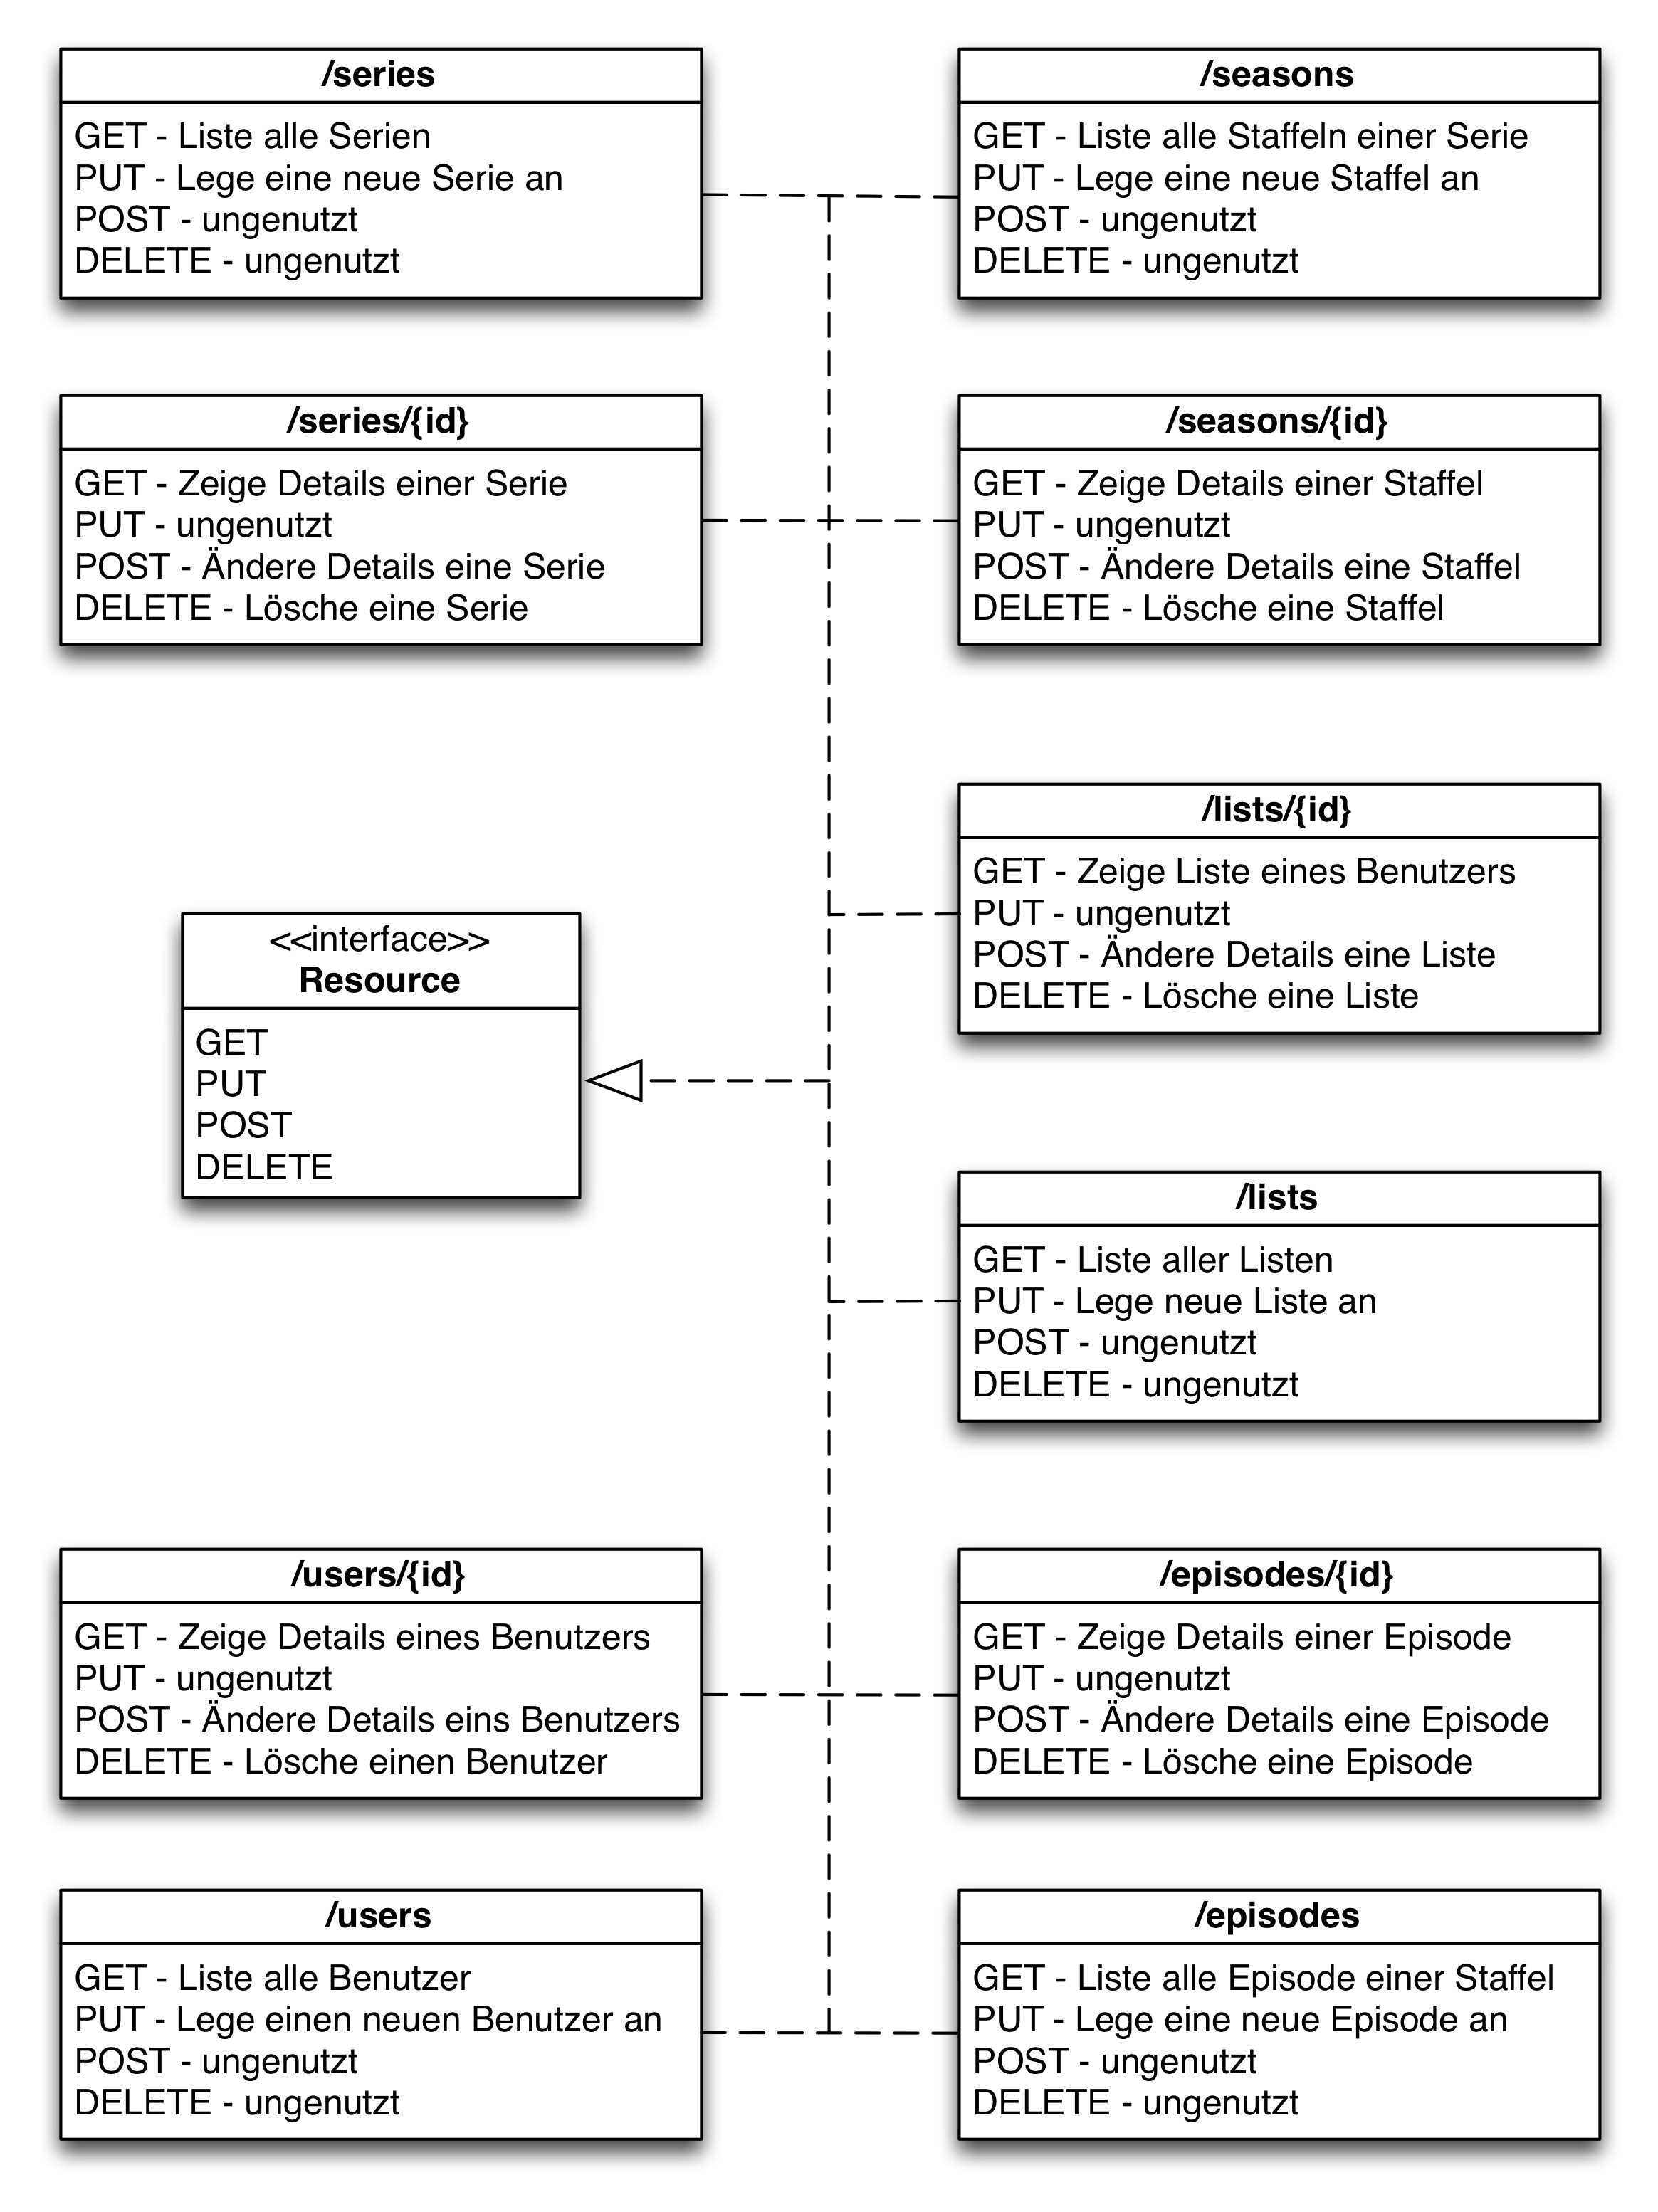
\includegraphics[width=1\textwidth]{images/bedeutunghttpmethoden.png}
\caption{Bedeutung der http Methoden}
\label{bedeutunghttpmethoden}
\end{figure}

\newpage


\subsection{RESTful Webservice}

\newpage

\subsection{Konzeption + XMPP Server einrichten}

\newpage

\subsection{XMPP - Client}

\newpage

\subsection{Client - Entwicklung}

\newpage

\section{Projektreflektion}

\newpage

\listoffigures

\newpage

\listoftables


\end{document}
